\section{Nombre: Mictlantecutli}  \label{per:mictlantecutli}
\subsection{Descripción:}   
Su figura es la de un esqueleto cuya calavera esta decorada con puntura morada de guerra. Porta un penacho de oro puro que refleja su condición como gobernante del Mictlán. El resto de su vestimenta emula una armadura de guerrero. Porta unas hombreras de oro con esmeraldas incrustadas, las hombreras se incrustan en un protector para el pecho que tiene diferentes grabados, mientras que sus protectores para los brazos están hechos de esmeraldas. Usa un taparrabo idéntico al que usan los tlatoanis, éste es sujetado por un delgado cinturón de oro. Mictlantechtli usa, ademas, una capa y zapatos característicos de quien es parte de la nobleza.
\\
\par
De carácter temperamental, le gusta tener el control de la situación por lo que es inusual verlo fuera de su zona de confort. Su ordenes son absolutas y no aceptara segundas opiniones, llegando incluso a destruir a aquellos que busquen alterar el orden. Desprecia las emociones humanas y considera que los humanos son criaturas pasionales y primitivas que no son conscientes del tiempo que tiene hasta que ya es tarde. Es un ser muy apegado a sus pertenencias. 
\subsection{Status:}
	\begin{itemize}
		\item Personaje no jugable.
		\item Enemigo jefe.
	\end{itemize}
\subsection{Imagen}
Ver figura \ref{fig:MictlantechtliDiseno}
	\begin{figure}
					\centering
					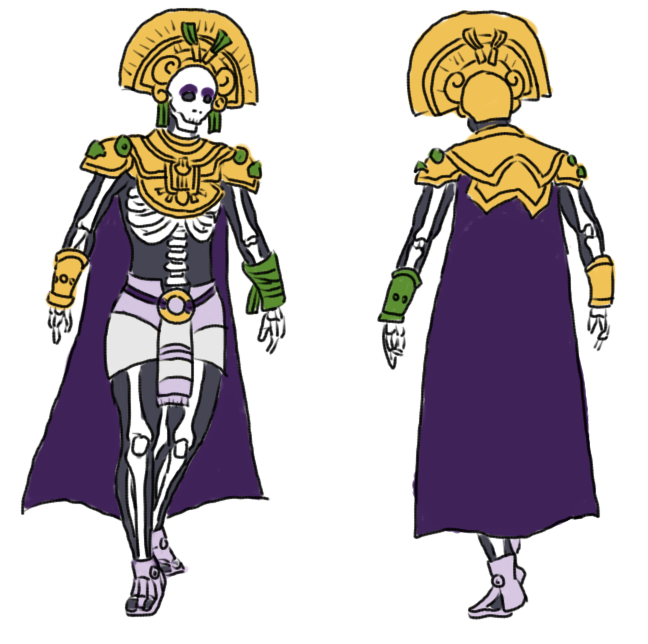
\includegraphics[height=0.3 \textheight]{Imagenes/ReyInframundo}
					\caption{Concepto de diseño de Mictlantechtli.}
					\label{fig:MictlantechtliDiseno}
	\end{figure}
\subsection{Concepto:}
\begin{itemize}
	\item \textbf{Historia antes del juego:}
	Después de la creación del quinto Sol,  Mictlantechtli se negó a dar los huesos de los antiguos hombres para rehacer la humanidad, pues consideraba que la humanidad como un capricho de Quetzalcóatl. Si bien al final termina ayudando, nunca perdonara que Quetzalcóatl y Xólotl robaron los huesos de los antiguos hombres del inframundo.
	\\
	\par
	El nuevo orden que instauran los dioses con el quinto sol, trae nuevas responsabilidades para  Mictlantechtli. Su rol no solo sería garantizar la purificación de las almas de los muertos, ahora también debería encargarse de la seguridad de los trece cielos al evitar que cualquiera pudiera entrar al Mictlán. Por consejo de  Mictecacíhuatl,  Mictlantechtli le exige a los dioses gobernantes de los trece cielos la presencia de nuevos guardianes para los niveles del Inframundo; desafortunadamente no todos los aspirantes logran pasar los requisitos de Mictecacíhuatl y  Mictlantechtli, por lo que Mictlantechtli toma los huesos de diferentes animale smuertos y crea a Xochitónal. Completando así los nueve guardianes.
	\\
	\par
	Luego del exilio de Quetzalcóatl, Mictlantechtli le deja en claro a Tezcatlipoca que a él le da igual quien gobierne los trece cielos siempre que él sea quien gobierne el Mictlán, advirtiendole que él no va a tolerar que se desate una guerra civil entre los dioses por los conflictos entre Tezcatlipoca y Quetzalcóatl. 
	\item \textbf{Historia durante el juego:}
	La muerte de Xochitónal toma por sorpresa a Mictlantechtli, pero debe de dejar a un lado el poco afecto que tenía por su creación para dar nuevas ordenes para mantener el orden de sus dominios. A medida de que cada uno de los guardianes va cayendo en el campo de batalla,  Mictlantechtli comienza a aceptar la derrota, sin embargo su orgullo le impide aceptarlo abiertamente. 
	\item \textbf{Relaciones:}
	\begin{itemize}
		\item \textbf{Mictecacíhuatl:} Esposa de Mictlantechtli. El lazo matrimonial que los une no es producto del amor, sino del deber. Ambos dioses colaboran juntos para mantener en orden el Mictlán. Si bien Mictlantechtli no ama a su esposa, si tiene un gran afecto y respeto. Este afecto lo lleva a pedirle a  Mictecacíhuatl que se retire del inframundo y vaya a los trece cielos para mantenerla a salvo (ver aparatado \ref{per:mictecacihuatl}).
		
		\item \textbf{Quetzalcóatl:}  Mictlantechtli tiene un conflicto no resuelto con este dios, luego de que Quetzalcóatl robara los huesos de los antiguos hombres (ver aparatado \ref{per:quetzalcoatl}).
		
		\item \textbf{Xólotl:}  Desde el punto de vista de Mictlantechtli, Xólotl es un cobarde, resentido que busca alterar el orden por mera perversión (ver aparatado \ref{per:xolotl}).
		
		\item \textbf{Malinalli:}  Mictlantechtli ve en Malinalli una niña pequeña, asustada, obsesionada con las personas que ha perdido e incapaz de ver por si misma que Xólotl solo la utiliza (ver aparatado \ref{per:malinalli}). 
	\end{itemize}                     
\end{itemize}

\subsection{Encuentro:}
\begin{itemize}
	\item Su primera aparición es en la cinemática 9 (ver aparatado \ref{Cin:Cinematica09}).
	\item Como jefe, el jugador se enfrenta a él en el décimo nivel del juego (ver aparatado \ref{Nivel:Niv10}).
\end{itemize} 

\subsection{Habilidades:}
\begin{itemize}
	\item Todos los hombres del rey (ver aparatado \ref{hab.TodoRey})
	\item Fuego mortífero (ver aparatado \ref{hab.FuegoMor}).
	\item Penitencia (ver aparatado \ref{hab.Penitencia}).
\end{itemize}  
\subsection{Armas:}
Sin armas.
\subsection{Ítems:}
Sin ítems
\subsection{Bloques de animación}     
	\begin{itemize}
		\item Etapa uno.
			\begin{itemize}
				\item Animación invocar a todos los hombres del rey.
				\item Animación disparar fuego mortífero.
				\item Animación invocar penitencia.
				\item Animación recibir daño.
				\item Animación morir.
			\end{itemize}
		\item Etapa dos.
			\begin{itemize}
				\item Animación lluvia de huesos.
				\item Animación estocada mortífera.
				\item Animación recibir daño.
				\item Animación morir.
			\end{itemize}
		\item Etapa tres.
			\begin{itemize}
				\item Animación Dispara burbujas.
				\item Animación invocar lluvia de rocas.
				\item Animación disparar fuego.
				\item Animación disparar raíz diablo.
				\item Animación lanzar lava.
				\item Animación recibir daño.
				\item Animación morir.
			\end{itemize}				 
	\end{itemize}